\documentclass[12pt]{article}
\usepackage[utf8]{inputenc}
\usepackage[UTF8]{ctex}
\usepackage{biblatex}
\usepackage{amssymb}
\usepackage{latexsym}
\usepackage{amsmath}
\usepackage{cases}
\usepackage{geometry}
\usepackage{graphicx}
\usepackage{float}
\usepackage{listings}
\usepackage{enumerate}
\usepackage{color}

\usepackage{algorithm}
\usepackage{algorithmic}

% 调整目录间距的宏包
\usepackage{setspace}

\usepackage{multirow}
\usepackage{float}
\usepackage{fancyhdr}  % header,footer的设置

\newcommand{\subsubsubsection}[1]{\paragraph{#1}\mbox{}\\}
\setcounter{secnumdepth}{4} % how many sectioning levels to assign numbers to
\setcounter{tocdepth}{4} % how many sectioning levels to show in ToC

% 封面的相关命令设置
\newcommand{\hmwkTitle}{Project 8 Model Order Reduction}
\newcommand{\hmwkClass}{《现代集成电路分析方法》}
\newcommand{\hmwkCompleteTime}{\today}
\newcommand{\hmwkAuthorName}{姓名:蔡志杰 }
\newcommand{\hmwMajor}{专业:电子科学与技术}
\newcommand{\hmwNumber}{学号:22112020002}
% 用fancyhdr设置header和footer
\pagestyle{fancy}
\lhead{\hmwkClass \hmwkTitle}
\rhead{蔡志杰 \quad 22112020002}
\cfoot{\thepage}


\addbibresource{bib.bib}
\setlength{\parindent}{0em}
\bibliography{bib}
\geometry{a4paper,scale=0.8}
\linespread{1.5}
\graphicspath{{Images/}}


%%%%%%%%%%%%%
%%% COVER %%%
%%%%%%%%%%%%%
\begin{document}

\begin{sloppypar}
\begin{titlepage}
\begin{center}



\includegraphics[scale = 0.9]{fudan.jpg}\\

\includegraphics[scale = 0.6]{fudan_logo.jpg}\\
\vspace{0.5in}
\linespread{1.9}\huge {\bfseries 现代集成电路分析方法}\\
\linespread{1.9}\LARGE {\bfseries \textbf{\hmwkTitle}}\\
\vspace{1.0in}
\large \hmwMajor{}\\
\large \hmwNumber{}\\
\large \hmwkAuthorName{}\\
% \large \date{\today} 

\end{center}
\end{titlepage}



%---------以下生成目录----------
\newpage
\begin{spacing}{1.2}
	\tableofcontents
\end{spacing}   % 若不想要目录, 注释掉该句
\thispagestyle{empty}   % 不要页眉页脚和页码
\newpage

%%%%%%%%%%%%%%%%%%%%%%%%%
%%% Problem Statement %%%
%%%%%%%%%%%%%%%%%%%%%%%%%
\section{题目}
\qquad 请设计一个程序,用AWE 或PRIMA方法(见refernce目录论文)对某线性电路系统进行MOR(Model Order Reduction,模型降阶)。原始系统阶数为m,其MNA方程为,:
\begin{equation}
\label{MNA1}
C \dot{x}(t)+G x(t)=B u(t)
\end{equation}
\begin{equation}
  \label{MNA2}
y=L^T x(t) 
\end{equation}
 
\qquad 降阶后的系统阶数为$n(n < m)$,表示为:

\begin{equation}
  \label{MNA_reduced}
  \widetilde{C} \dot{z}(t)+ \widetilde{G} z(t) = \widetilde{B} u(t)
\end{equation}
\begin{equation}
  y=\widetilde{L^T} z(t) 
\end{equation}

\qquad 程序应该能处理MIMO系统。


\subsection{输入}
\qquad (1)电路方程:以提供的stamp程序的输出作为本程序的输入。 \par
\qquad (2)降阶系统阶数$n$和展开点$s_0$。 \par

\subsection{输出结果}
\qquad 程序应生成$\widetilde{C},\widetilde{G},\widetilde{B},\widetilde{L^T}$四个矩阵,并以适当的形式保存成文件。此外测试用例还要求一些额外的输出,参见后面部分的说明。\par

\subsection{提交结果}
\qquad 程序建议采用MATLAB完成,需提交以下内容: \par
\qquad (1) 源程序,应有必要的注释。 \par
\qquad (2) 使用除MATLAB外其他语言的,需要提交最终编译的可执行代码。 \par
\qquad (3) 一份完整的说明,主要内容包括:主要设计思想,程序结构,编译的环境和方法,运行的环境和方法,输入的格式或方法,以及其他需要特别说明的地方。 \par
\qquad (4) 对测试用例的测试结果和分析。 \par

\subsection{测试用例}
\qquad Benchmark目录下提供1个测试用例PEEC.mat。

\qquad PEEC.mat原始系统为一个SISO系统,阶数m = 306。PEEC.mat文件包含了原始系统MNA方程中的四个矩阵。该文件为MATLAB 格式,可以在MATLAB 命令行方式下用以下命令载入:

\qquad > > load PEEC.mat;

\qquad 程序应对该系统进行降阶,并以适当的方式对降阶过程和降阶系统进行评估。

\qquad (1) 做图:比较降阶系统传输函数 $\left| \tiled{H}(s) \right|$ 与原始系统传输函数 $|H(s)|$ 。 \par
\qquad (2) 做图:给出降阶系统与原始系统的传输函数在不同s处的误差。 \par
\qquad (3) 对上图在20000个点上采样,计算最大绝对误差和均方绝对误差。均方误差的定义: $MSE=\sqrt{\frac{1}{p} \sum_{i=1}^p E_i^2}$ ,其中$E_i$为每个采样点上的误差,$p$为采样点数。 \par
\qquad (4) 分别给出降阶过程的时间,求解原系统的时间,求解降阶系统的时间。适当改动展开点s0和降阶阶数n,观察对得到的降阶系统的影响,并进行分析。 \par
\qquad 一些建议或提示: \par
\qquad (A) 求解原始系统和降阶系统可以采用在频域每个采样点上求解代数方程的方法。降阶系统有一些特殊的性质,可以加以利用以提高求解速度。 \par
\qquad (B) 由于计算原始系统传输函数比较耗费时间,建议只计算一次,将结果保存下来,在以后每次运行程序时作为输入读入即可。 \par
\qquad (C) 一组供参考的输入参数:n = 60,s0 = $2\pi \times 10^9$ 。传输函数观察0 – 15 GHz区间。 \par


%%%%%%%%%%%%%%%%%
%%% Algorithm %%%
%%%%%%%%%%%%%%%%%
\newpage
\section{算法原理}

\qquad 对于复杂的电路系统,采用模型降阶的方法通常可以大量减小矩阵运算的复杂度。对矩阵降阶的方法主要有两种AWE和PRIMA,AWE的思想是通过对传输函数进行泰勒展开,然后通过将降阶后的传输函数与原始传输函数进行矩匹配来得到降阶后的传输函数,但是其不具有数值稳定性也无法保证无源性。PRIMA方法是基于Arnoldi方法采用合同变换保证了系统的无源性。故本文采用PRIMA方法对模型进行降阶。接下来介绍一下AWE和PRIMA方法的算法原理。


\subsection{Asymptotic Waveform Evaluation,AWE}
\qquad AWE \cite{1}采用的主要思路是先给出降阶后的传输函数公式,然后通过与原始传输函数泰勒展开后的结果进行矩(Moment)匹配来求解降阶后的传输函数。对于公式(\ref{MNA1})和(\ref{MNA2})所示的状态方程进行拉普拉斯变换可得如下公式:
\begin{equation}
  \begin{align}
    & CsX(s) + GX(s) = BU(s) \\
    & \qquad Y(s) = L^TX(s) \\
  \end{align}
\end{equation}
\begin{equation}
  H(s) = \frac{Y(s)}{U(s)} = \frac{L^{T} C^{-1} B}{sI + C^{-1}G} = m_0 + m_{1}s + m_{2}s^{2} + \ldots
\end{equation}

\qquad 在s=0点处展开
\begin{equation}
  m_0=H(s)|_{s=0}=L^{T}\left(\frac{C^{-1}}{sI + C^{-1}G}\right)|_{s=0} C^{-1} B = L^{T} \cdot (C^{-1}G)^{-1} \cdot  C^{-1} B 
\end{equation}
\begin{equation}
  m_1= \frac{dH(s)}{ds} |_{s=0} = L^{T} \left( \frac{C^{-1}}{sI + C^{-1}G} \right)^{'} |_{s=0} C^{-1} B = - L^{T} \cdot (C^{-1}G)^{-2} \cdot C^{-1} B 
\end{equation}

\qquad 递推可得:
\begin{equation}
  m_i=\frac{d^i H(s)}{ds^i}|_{s=0}  = - L^{T} \cdot (C^{-1}G)^{-i-1} \cdot  C^{-1} B 
\end{equation}

\qquad 假设降阶后的传输函数为:
\begin{equation}
  \hat{H}(s)=\frac{\hat{b}_0+\hat{b}_1 s+\ldots+\hat{b}_{q-1} s^{q-1}}{1+\hat{a}_1 s+\ldots+\hat{a}_q s^q}
\end{equation}
\begin{equation}
  \hat{H}(s)=\hat{m}_0 + \hat{m}_1 s  + \hat{m}_2 s^2 + \ldots 
\end{equation}

\qquad 令$\hat{m_i} = m_i, 0 \le i < 2q$进行矩匹配,可得如下方程组,进而可以求解降阶后的传输函数系数。
\begin{equation}
  \hat{H}(s)=\frac{\hat{b}_0+\hat{b}_1 s+\ldots+\hat{b}_{q-1} s^{q-1}}{1+\hat{a}_1 s+\ldots+\hat{a}_q s^q} =\hat{m}_0 + \hat{m}_1 s  + \hat{m}_2 s^2 + \ldots + \hat{m}_{2q-1} s^{2q-1}
\end{equation}
\begin{equation}
  \begin{align}
    &\hat{b}_0=m_0 \\
    &\hat{b}_1=m_1+m_0 \hat{a}_1 \\
    &\vdots \\
    &\hat{b}_{q-1}=m_{q-1}+m_{q-2} \hat{a}_1+\ldots+m_0 \hat{a}_{q-1} \\
    &0=m_q+m_{q-1} \hat{a}_1+\ldots+m_0 \hat{a}_q \\
    &0=m_{q+1}+m_q \hat{a}_1+\ldots+m_1 \hat{a}_q \\
    &\vdots \\
    &0=m_{2 q-1}+m_{2 q-2} \hat{a}_1+\ldots+m_{q-1} \hat{a}_q \\
  \end{align}
\end{equation}

\qquad 由于AWE直接使用了$A^kb$作为Krylov子空间的基向量进行矩匹配,当$k$逐渐增大的时候会使得特征向量的方向趋向一致(接近最大特征值对应的特征向量的方向),因此无法保证数值稳定性,同时也无法保证模型的无源性(不出现右半平面的极点)。

\subsection{Passive Reduced-order Interconnect Macromodeling Algorithm}

\qquad PRIMA方法是在block arnoldi算法的基础上并采用合同变换来保证降阶后电路模型的无源性。Arnoldi算法将矩阵通过合同变换转换成一个阶数更小的上Hessenberg矩阵,其中转换矩阵$V$的列向量将张成一个Krylov子空间$closp V_q = span { v_1,v_2,\cdots,v_q }=K_q(A,b)=span { b,Ab,\cdots,A^{q-1}b }$,同时保证列向量彼此正交。由于Arnoldi算法是针对SISO(单输入单输出)系统(其中$b$和$L^T$都是一维的向量),block Arnoldi算法的提出解决了MIMO(多输入多输出)系统。接下来介绍PRIMA算法的具体原理和计算方法。

\qquad 根据系统状态方程在拉普拉斯域的表达形式,令$A \equiv -G^{-1}C, R \equiv G^{-1}B$,可得如下结果,注意这里的$B \in \mathbb{R}^{n \times N}$是一个矩阵其列数即为输出的数量,$n$为电路方程的未知数个数,$N$为电路的端口数(假设需要测量的端口与输入的电源信号数量相同都为$N$)。
\begin{equation}
  H(s)=L^T(G+sC)^{-1}B=L^T(I_n-sA)^{-1}R
\end{equation}

\qquad 将$H(s)$泰勒展开后的系数$M_i \in \mathbb{R}^{N \times N}$定义为block moment,可得$M_i = L^T A^i R$。 关于矩阵$A \in \mathbb{R}^{n \times n}, R = [r_0\ r_1\ \cdots \ r_N]$的block Krylov 空间定义为:
\begin{equation}
  Kr(A, R, q) \equiv colsp \left[R, A R, A^2 R, \cdots,A^{k-1} R, R^k r_0, R^k r_1, \cdots, A^k r_l\right] \ k=\lfloor q / N\rfloor, \quad l=q-k N .
\end{equation}

\qquad block Arnoldi算法将系统函数$A$降阶成一个更小的上Hessenberg矩阵$H_p$。算法会不断迭代来求解$X$的列向量,使其满足$AX=XH_q,X^TX=I_q,X \in \mathbb{R}^{x \times q}$,可以将$X$看作一个Krylov空间$Kr(A,R,q)$的正交子空间。令$x_n = Xz_q, z_q \in \mathbb{R}^{q \times 1}$进而可以得到下式:
\begin{equation}
  \begin{aligned}
    & -X^T G^{-1} C X \dot{z}_q = X^T X z_q-X^T G^{-1} B u_N \\
    & \qquad \qquad \qquad Y_N =L^T X z_q \\
  \end{aligned}
\end{equation}

\qquad 进而可得:
\begin{equation}
  \begin{align}
    & H_q \dot{z}_q =z_q-X^T R u_N \\
    & \qquad Y_N =L^T X z_q \\    
  \end{align}
\end{equation}

\qquad 降阶后的传输函数为:
\begin{equation}
  \hat{H}(s)=L^T X\left(I_q-s H_q\right)^{-1} X^T R
\end{equation}

\qquad 可以证明降到$q$阶后,满足$A^i R=X H_q^i X^T R, \quad 0 \leq i< \lfloor\frac{q}{N} \rfloor$,即前
$\lfloor \frac{q}{N} \rfloor$个block moments是和原始传输函数匹配的。降阶后的阶数越大,得到的系统便越接近原始系统。

\qquad Arnoldi系列方法中都是直接对整个系数矩阵$G^{-1}C$进行降阶。而在PRIMA方法中将对每一个矩阵单独进行降阶来保证无源性,
\begin{equation}
  \begin{align}
    & \left(X^T C X\right) \dot{\tilde{x}}_q =-\left(X^T G X\right) tilde{x}_q+\left(X^T B\right) u_N \\
    &\qquad \qquad \qquad Y_N =\left(L^T X\right) \dot{\tilde{x}}_q \\
  \end{align}
\end{equation}
\begin{equation}
  \tilde{C}=X^T C X,\  \tilde{G}=X^T G X, \ \tilde{B}=X^T B, \ \tilde{L}=X^T L .
\end{equation}

\qquad 降阶后的传输函数即为:
\begin{equation}
\label{hhat}
  \hat{H}(s)=\tilde{L}^T \left(\tilde{G} + s \tilde{C} \right)^{-1} \tilde{B}
\end{equation}

\qquad 论文中证明了PRIMA对系统无源性的保证以及系统的矩匹配,详细证明可参见\cite{2}。

\qquad 前面提到的方法都是基于$s=0$进行泰勒展开,当展开点为$s_0$时,可得如下的传输函数:
\begin{equation}
  H(s)=L^T\left[I+\left(s-s_0\right)\left(C s_0+G\right)^{-1} C\right]^{-1}\left(C s_0+G\right)^{-1} B
\end{equation}

令$A=-\left(C s_0+G\right)^{-1} C, R=\left(C s_0+G\right)^{-1} B$,上式可化简为:
\begin{equation}
  H(s)=L^T\left[I-\left(s-s_0\right) A\right]^{-1} R
\end{equation}

\qquad PRIMA方法的降阶流程:
\begin{algorithm}
  \caption{PRIMA generate transform matrix X} % 名称
  \label{alg:PRIMA}
  \begin{algorithmic}[1]
  % \REQUIRE guide range $guide$, pins of net $pins$.
  % \ENSURE routing connections $connections$. \\
      \STATE Set$\left[\mathbf{b}_1\left|\mathbf{b}_2\right| \ldots \mid \mathbf{b}_{\mathrm{N}}\right]=\mathbf{B}$ and $\left[\mathbf{I}_1\left|\mathbf{I}_2\right| \ldots \mid \mathbf{1}_{\mathrm{N}}\right]=\mathbf{L}$
      \STATE Solve $()\mathbf{G} + s_0 \mathbf{C}) \mathbf{R}=\mathbf{B}$ for $\mathbf{R}$
      \STATE $\left(\mathbf{X}_0, \mathbf{T}\right)=qr(\mathbf{R}) ; \# qr factorization of \mathbf{R}$
      \STATE If $\frac{q}{N}$ is not an integer, set $n=\left\lfloor\frac{q}{N}\right\rfloor+1$, else set $n=\frac{q}{N}$
      \STATE For $k=1,2, \ldots, n$
      \STATE \qquad Set $\mathbf{V}=\mathbf{C X}_{k-1}$
      \STATE \qquad Solve $\mathbf{G} \mathbf{X}_k^{(0)}=\mathbf{V}$ for $\mathbf{X}_k^{(0)}$
      \STATE \qquad For $j=1, \ldots, k$
      \STATE \qquad \qquad $\mathbf{H}=\mathbf{X}_{k-j}^T \mathbf{X}_k^{(j-1)} $
      \STATE \qquad \qquad $\mathbf{X}_k^{(j)}=\mathbf{X}_k^{(j-1)}-\mathbf{X}_{k-j} \mathbf{H} $
      \STATE \qquad $\left(\mathbf{X}_k, \mathbf{T}\right)=q r\left(\mathbf{X}_k^{(k)}\right) ; q r \text { factorization of } \mathbf{X}_k^{(k)}$
      \STATE Set $\mathbf{X}=\left[\mathbf{X}_0 & \mathbf{X}_1 & \ldots & \mathbf{X}_{k-1}\right]$ and truncate $\mathbf{X}$ so that it has $q$ columns only.
  
  \end{algorithmic}
\end{algorithm}

\qquad 根据得到的转换矩阵X对传输函数进行降阶可得到如下公式:
\begin{equation}
  H(s)=L^T X\left[I+s_0 X^T A X-s X_T A X\right]^{-1} X^T R
\end{equation}

\qquad 与原始的传输函数公式(\ref{hhat})对比, 可得到降阶后的矩阵为:
\begin{equation}
\label{r}
  \begin{align}
    & \tilde{C}=-X^T A X \\ 
    & \tilde{G}=I+s_0 X^T A X \\
    & \tilde{B}=X^T R \\ 
    & \tilde{L}^T=L^T X \\
  \end{align}
\end{equation}

\newpage
\section{算法实现}
\subsection{算法流程}
\qquad 算法流程
\begin{itemize}
  \item 加载预先生成好的电路方程矩阵文件PEEC.mat(若为输入为电路方程可使用stamp函数对电路方程进行解析,得到MNA方程的相关矩阵,与之前的pj相同)。(main.m)
  \item 求解原始电路方程传输函数的频率响应,并保留数据。(freq\_respond.m)
  \item 根据设定的阶数、展开点频率以及原始电路方程的矩阵求解PRIMA降阶后的矩阵。(prima.m)
  \item 求解降阶后电路方程传输函数的频率响应,并保留数据。(freq\_respond.m)
  \item 根据原始电路频响和降阶电路频响进行作图对比。(main.m)
  \item 采用网格法尝试一系列模型阶数和展开点频率的降阶过程,对比不同参数设置下仿真的误差情况以及运行时间。(compare.m)
\end{itemize}

\subsection{模型降阶与传输函数频响计算}

\qquad 模型降阶的方法可以分为两个步骤,第一步是计算转换矩阵$X$,详细的计算方法及流程可以参见Algorithm \ref{alg:PRIMA},之后根据公式(\ref{r})计算降阶后的各个系数矩阵。

\qquad 传输函数频率响应的计算可以依照公式$H(s)=L^T(G+sC)^{-1}B$,在各个采样频率点计算得到相应频带的频响特性。其中需要注意的一点是由于需要能解决MIMO的系统,$B \in \mathbb{R}^{n \times \#input}, L^T \in \mathbb{R}^{\#output \times n}$都是二维矩阵,其中$n, \#input, \#output$分别为电路方程中的未知数、电路的输入端口和电路的输出端口数量。因此计算得到的传输函数也是一个矩阵,为了方便后续对误差的计算和结果对比,将传输矩阵二维的结果以一维的形式存储(原始的二维索引转换成相应的一维索引,即(i,j)=>i+(j-1)*#row,其中i对应输出的端口序号,j对应输入的端口序号)。最后输出的对比图像目前选则第一个输入对第一个输出的传输函数的频响(可以通过修改main.m函数中第50、58行的输出数据序号)。

\subsection{输出}
\qquad 为了方便对比降阶前后电路系统的频响特性,将运行后的相关结果(运行时间、频响特性)通过save命令存储到.mat文件中(文件在Benchmark目录下,origin\_system.mat存储了原始系统的相关数据,reduced\_result.mat存储了降阶后的相关数据,compare.m存储了网格测试实验的数据)。

\subsection{编译与运行}
\qquad 程序基于Matlab 2015b(32位)平台,将电路模型降阶、系统频率响应求解和对比结果输出的过程都打包在main函数中。可以在Benchmark或src目录中运行main函数(两个目录中都含有相关的代码文件和benchmark——PEEC.mat)。main函数的接口为$main(order, f0, fs, fe, sampleNum)$.其中order为模型降阶的目标阶数,f0为泰勒展开点频率,[fs,fe]为求解频响特性的频率区间, sampleNum为频响特性中采样的点数。下面给出一个运行示例:
\begin{equation}
  main(60, 1e9, 0, 1.5e10, 20000)
\end{equation}

\section{结果与分析}
\subsection{实验结果}
\qquad 实验设置:频响特性的频率区间为[0Hz,15GHz],区间采样点设置为20000,对于阶数和展开点的选取后续将分别排列组合出9组搭配并展示结果频响结果和误差。之后还会进行更加细致的网格测试,模型阶数从10到200阶,以10作为递增的步长。同时展开点从1GHz到15GHZ以1GHz为递增的步长,分别测试排列组合出的300种参数,并记录运行结果的误差和运行时间,最后以三维网格图的形式进行呈现。(为了更加直观地展示运行时间的变换,记录程序运行时的cpu time而非elapsed time,cpu时间将不考虑并行的加速效果)

\subsubsection{30阶,展开点1e6的运行结果}
\begin{figure}[H]
  \centering
  \includegraphics[width=0.9\columnwidth]{figure/30\_1e6.png}
  \caption{30阶,展开点1e6的运行结果}
\end{figure}

\subsubsection{30阶,展开点1e8的运行结果}
\begin{figure}[H]
  \centering
  \includegraphics[width=0.9\columnwidth]{figure/30\_1e8.png}
  \caption{30阶,展开点1e8的运行结果}
\end{figure}

\subsubsection{30阶,展开点1e10的运行结果}
\begin{figure}[H]
  \centering
  \includegraphics[width=0.9\columnwidth]{figure/30\_1e10.png}
  \caption{30阶,展开点1e10的运行结果}
\end{figure}


\subsubsection{60阶,展开点1e6的运行结果}
\begin{figure}[H]
  \centering
  \includegraphics[width=0.9\columnwidth]{figure/60\_1e6.png}
  \caption{60阶,展开点1e6的运行结果}
\end{figure}

\subsubsection{60阶,展开点1e8的运行结果}
\begin{figure}[H]
  \centering
  \includegraphics[width=0.9\columnwidth]{figure/60\_1e8.png}
  \caption{60阶,展开点1e8的运行结果}
\end{figure}

\subsubsection{60阶,展开点1e10的运行结果}
\begin{figure}[H]
  \centering
  \includegraphics[width=0.9\columnwidth]{figure/60\_1e10.png}
  \caption{60阶,展开点1e10的运行结果}
\end{figure}


\subsubsection{120阶,展开点1e6的运行结果}
\begin{figure}[H]
  \centering
  \includegraphics[width=0.9\columnwidth]{figure/120\_1e6.png}
  \caption{120阶,展开点1e6的运行结果}
\end{figure}

\subsubsection{120阶,展开点1e8的运行结果}
\begin{figure}[H]
  \centering
  \includegraphics[width=0.9\columnwidth]{figure/120\_1e8.png}
  \caption{120阶,展开点1e8的运行结果}
\end{figure}

\subsubsection{120阶,展开点1e10的运行结果}
\begin{figure}[H]
  \centering
  \includegraphics[width=0.8\columnwidth]{figure/120\_1e10.png}
  \caption{120阶,展开点1e10的运行结果}
\end{figure}


\subsubsection{网格测试结果}
\qquad 实验设置:频响特性的频率区间为[0Hz,15GHz],区间采样点设置为20000,对于阶数和展开点的选取后续将分别排列组合出9组搭配并展示结果频响结果和误差。之后还会进行更加细致的网格测试,模型阶数从10到200阶,以10作为递增的步长。同时展开点从1GHz到15GHZ以1GHz为递增的步长,分别测试排列组合出的300种参数,并记录运行结果的误差和运行时间。结果如下图所示:
\begin{figure}[H]
  \centering
  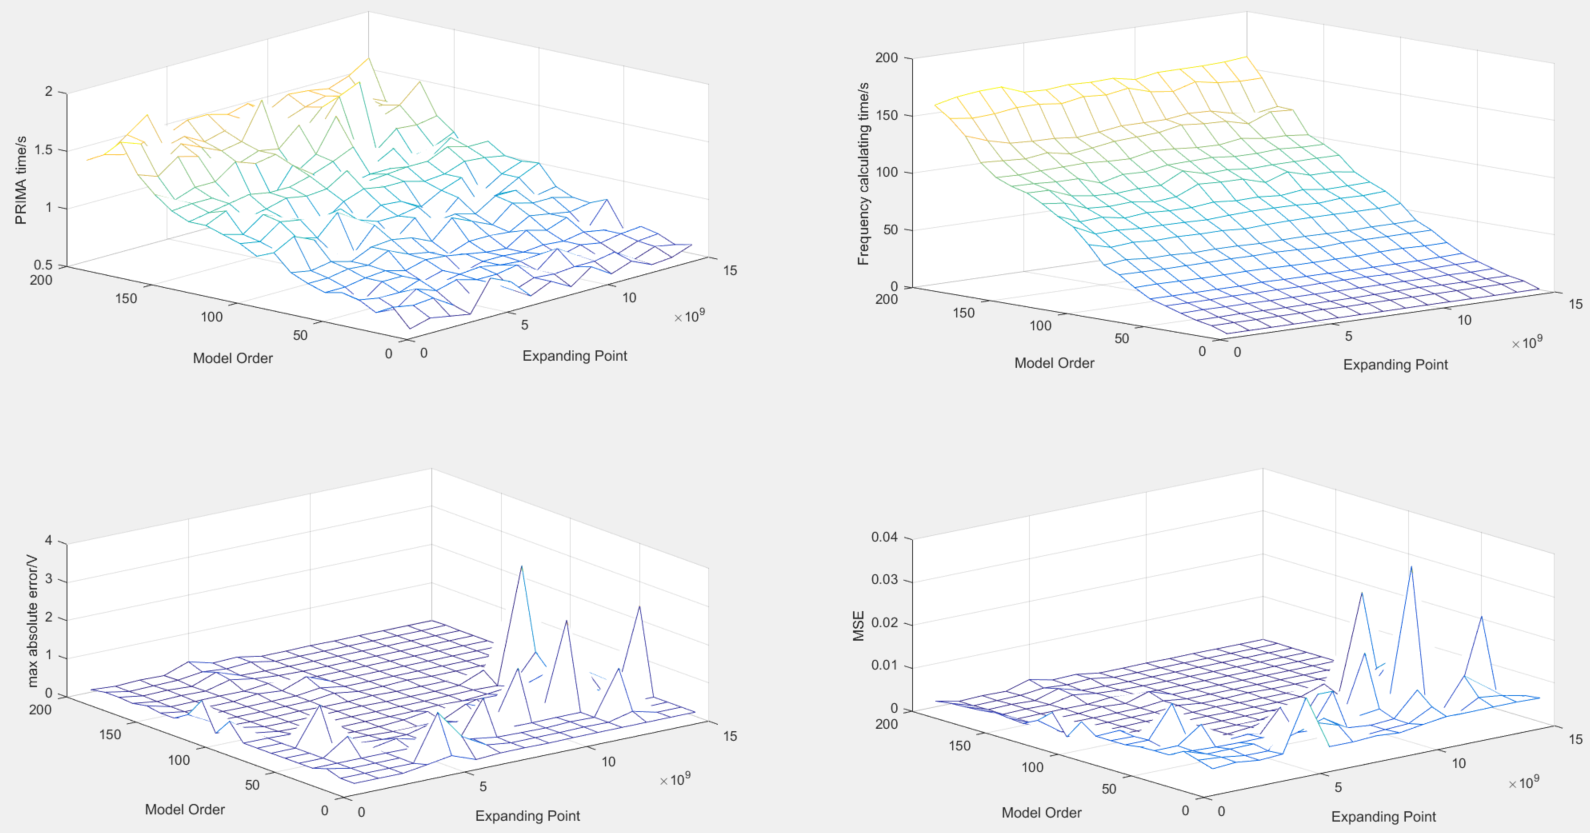
\includegraphics[width=0.9\columnwidth]{figure/comparison.png}
  \caption{网格测试结果}
\end{figure}

\subsection{结果分析}
\qquad 首先根据实验结果可以看出系统降阶确实可以很大程度地加速。根据九组参数的实验结果可以知道在固定降阶阶数的时候,选择不同的展开点对系统频响影响较大,越接近展开点的频段误差越小,准确度越高;对于固定展开点的情况,降阶阶数越大得到的频响特性越准确,均方误差越小。在9组实验中降阶到120阶,展开点在10GHz的时候得到的结果误差最小,这是由于原始系统是一个高通滤波器,通带主要集中在1GHz到10GHz。

\qquad 根据网格测试的结果可以看出随着阶数的增加PRIMA降阶时间也不断增加,同时计算降阶后系统频响的运行时间也不断增加,且通过观察两者的增长趋势接近线性。根据均方误差的分布可以看出除了一些波动的情况,整体趋势是随着降阶阶数的增加而减小,同时在展开点中4GHz-9GHz这一频段的误差更小。


\section{文件结构}
\begin{itemize}
  \item main.m:包含MOR中模型降阶、系统频响求解和结果对比的代码。
  \item freq\_respond.m:根据给定参数和电路模型求解系统频响。
  \item prima.m:根据给定系数,实现系统降阶。
  \item compare.m:实现网格测试以及结果展示。
\end{itemize}

\end{sloppypar}
\begin{thebibliography}{99}  

  \bibitem{1}Pillage L T, Rohrer R A. Asymptotic waveform evaluation for timing analysis[J]. IEEE transactions on computer-aided design of integrated circuits and systems, 1990, 9(4): 352-366.
  \bibitem{1}Odabasioglu A, Celik M, Pileggi L T. PRIMA: Passive reduced-order interconnect macromodeling algorithm[J]. IEEE Transactions on computer-aided design of integrated circuits and systems, 1998, 17(8): 645-654.
  \end{thebibliography}

\end{document}